\documentclass[]{article}
\usepackage[utf8]{inputenc}
\usepackage{hyperref}
\usepackage[spanish]{babel}
\usepackage{listings}
\usepackage{xcolor} %para el texto con coloresç
\usepackage{tocloft}
\usepackage{graphicx}

\usepackage[colorinlistoftodos,prependcaption,textsize=tiny]{todonotes}

\renewcommand{\cftsecleader}{\cftdotfill{\cftdotsep}} % Para que todo el índice tenga puntos
\newcommand{\code}[1]{{\lstinline[basicstyle=\ttfamily,mathescape]!#1!}}
\newcommand{\toolname}{\emph{Tutoriales Interactivos}}

\lstset{ %
	%backgroundcolor=\color{white},  % choose the background color; you must add \usepackage{color} or \usepackage{xcolor}
	basicstyle=\sffamily,      % the size of the fonts that are used for the code
	breakatwhitespace=false,         % sets if automatic breaks should only happen at whitespace
	breaklines=true,                 % sets automatic line breaking
	captionpos=none,                 % sets the caption-position to bottom
	commentstyle=\itshape\color{gray},           % comment style
	%deletekeywords={...},           % if you want to delete keywords from the given language
	escapeinside={(*}{*)},           % if you want to add LaTeX within your code
	extendedchars=true,              % lets you use non-ASCII characters; for 8-bits encodings only, does not work with UTF-8
	frame=tb,	                   % adds a frame around the code
	keepspaces=true,                 % keeps spaces in text, useful for keeping indentation of code (possibly needs columns=flexible)
	columns=fullflexible,
	%keywordstyle=\color{blue},      % keyword style
	keywordstyle=\sffamily\color{teal},
	numbers=left,                    % where to put the line-numbers; possible values are (none, left, right)
	numbersep=5pt,                   % how far the line-numbers are from the code
	numberstyle=\tiny, % the style that is used for the line-numbers
	%rulecolor=\color{black},         % if not set, the frame-color may be changed on line-breaks within not-black text (e.g. comments (green here))
	showspaces=false,                % show spaces everywhere adding particular underscores; it overrides 'showstringspaces'
	showstringspaces=false,          % underline spaces within strings only
	showtabs=false,                  % show tabs within strings adding particular underscores
	stepnumber=1,                    % the step between two line-numbers. If it's 1, each line will be numbered
	stringstyle=\color{blue},     % string literal style
	tabsize=2,	                   % sets default tabsize to 2 spaces
	title=\lstname,                   % show the filename of files included with \lstinputlisting; also try caption instead of title	
	mathescape=true
}

% Title Page
\title{\toolname{} - Manual de usuario \\ \emph{(Borrador)}}
\author{Enrique Martín Martín$^a$ (\url{emartinm@ucm.es}) \\ 
	Salvador Tamarit$^b$ (\url{stamarit@dsic.upv.es}) \\
	\emph{Revisor:} Jaime Sánchez Hernández$^a$ (\url{jaime@sip.ucm.es}) \\~\\[-.4cm]
	\normalsize{\emph{$^a$Dpto. de Sistemas Informáticos y Computación}}\\[-0.1cm]
	\normalsize{\emph{Fac. Informática, Universidad Complutense de Madrid}}\\[-0.1cm]
	%\normalsize{\emph{C/ Profesor José García Santesmases, 9. 28040 Madrid, Spain}}\\[-0.1cm]
	\normalsize{\emph{$^b$Dep. Sistemes Informàtics i Computació}}\\[-0.1cm]
	\normalsize{\emph{Universitat Politècnica de València}}\\[-0.1cm]
	%\normalsize{\emph{Camí de Vera, s/n. 46022 València}}\\[-0.1cm]
}


\begin{document}
\maketitle

\tableofcontents

\clearpage

\section{Instalación y ejecución}\todo{Enrique}

Para poder ejecutar la herramienta \toolname{} debéis tener instalada en vuestro sistema la última versión de Java (en el momento de escribir este manual es la \emph{versión 8 update 131)}. Para ello debéis acceder a la página \url{https://www.java.com/es/download/} y seguir las instrucciones.

Una vez disponemos de la última versión de Java, la instalación de la herramienta \toolname{} es muy sencilla: únicamente es necesario descargar el programa junto con las lecciones y situarlo en alguna carpeta del sistema (por ejemplo el directorio personal o el escritorio). Si vais a utilizar \toolname{} es una asignatura, lo más probable es que el profesor os proporcione un fichero comprimido con todos los elementos incorporados. En el caso de no disponer de este fichero comprimido proporcionado por el profesor, podéis descargar la herramienta de su repositorio oficial: \url{https://github.com/emartinm/TutorialesInteractivos/archive/master.zip}.
% y descomprimirlo en alguna carpeta del sistema\footnote{Si disponéis del sistema de control de versiones \emph{GIT} también podréis clonar el repositorio de la herramienta  usando la dirección \url{https://github.com/emartinm/TutorialesInteractivos.git}}.

Para ejecutar la herramienta, únicamente hay que hacer doble clic en el fichero \texttt{TutorialesInteractivos-jar-with-dependencies.jar} situado en la carpeta \texttt{target} dentro del directorio principal de la herramienta. En caso de no poder iniciar la herramienta de esta manera consulta la sección~\ref{sec:problemas_arrancar}.

\section{Configuración de la aplicación}\todo{Enrique}

La primera vez que se inicia la herramienta se acceder directamente a la ventana de configuración (ver figura~\ref{fig:config1}).
%
\begin{figure}[tbp]
\begin{center}
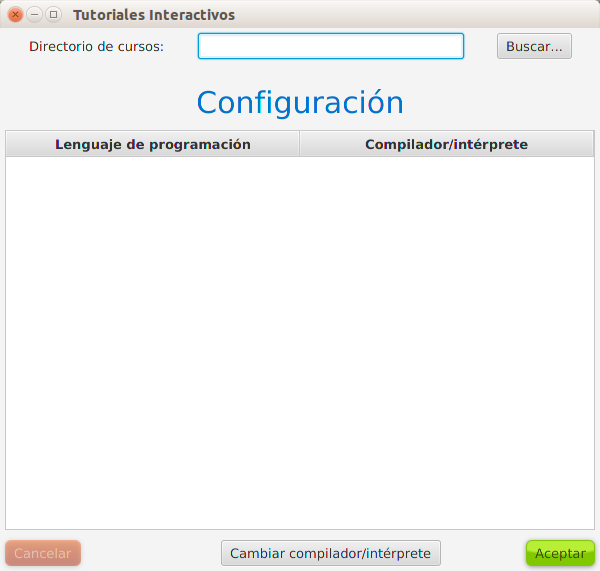
\includegraphics[scale=0.4]{Configuracion_vacia.png}
\end{center}
\caption{Ventana inicial de configuración\label{fig:config1}}
\end{figure}
%
En esta ventana lo primero que hay que hacer es configurar el \textbf{directorio de temas} pulsando el botón \emph{Buscar\ldots} que aparece aparece en la parte superior derecha. El directorio de temas normalmente se encuentra dentro del directorio principal de la herramienta, contiene carpetas por cada uno de los lenguajes disponibles: Python 3.x, C++, Java, etc. 

Tras configurar el directorio de temas, nos aparecerán varias entradas en el listado central de la ventana de configuración para establecer los compiladores o intérpretes para cada lenguaje disponible (ver figura~\ref{fig:config2}).
%
\begin{figure}[tbp]
\begin{center}
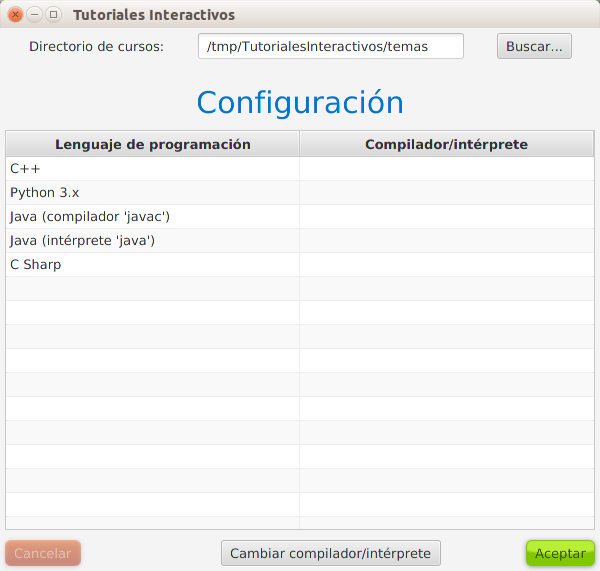
\includegraphics[scale=0.4]{Configuracion_lenguajes_vacio.png}
\end{center}
\caption{Ventana inicial de configuración con directorio de temas\label{fig:config2}}
\end{figure}
%


Al finalizar la configuración de la herramienta, la ventana debe tener un aspecto similar al mostrado en la figura~\ref{fig:config3}.

%
\begin{figure}[tbp]
\begin{center}
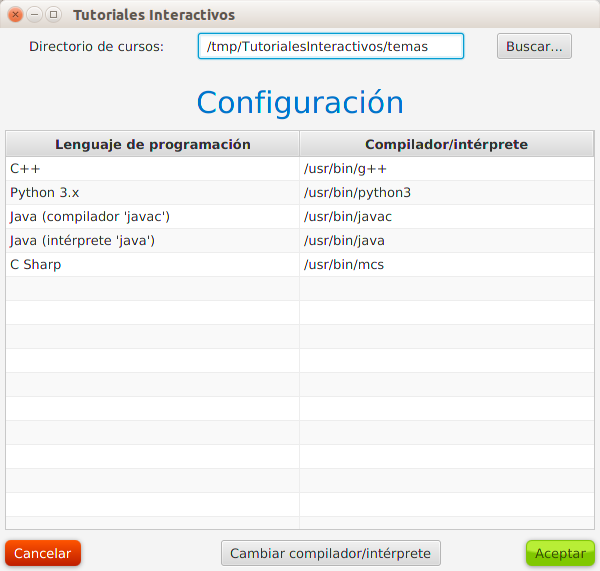
\includegraphics[scale=0.4]{Configuracion_lenguajes_relleno.png}
\end{center}
\caption{Ventana final configuración\label{fig:config3}}
\end{figure}
%
Ten en cuenta que \textbf{no es obligatorio configurar los compiladores o intérpretes de todos los lenguajes de programación disponibles}, únicamente de aquellos que vayas a utilizar para realizar tutoriales.

\todo{Explicación de la pantalla de configuración. Lenguajes soportados y diferencias linux-mac vs Windows (C\# y C++ a través de vcvars32.bat)}

\section{Navegación general}\todo{Tama}
Breve explicación de cómo llegar a una lección y los distintos apartados navegables

\section{Lecciones}\todo{Tama}
Navegación dentro de una lección. Distintas preguntas de una lección y qué hace cada botón

\section{Solución de problemas}\todo{Enrique}

\subsection{No puedo iniciar la herramienta}\label{sec:problemas_arrancar}
Si al hacer doble clic sobre el fichero \texttt{.jar} no se arranca la aplicación, comprueba que dicho fichero es \textbf{ejecutable}. Para ello abre el menú contextual con el botón derecho y explora las distintas opciones disponibles para cambiar los permisos del fichero.

Si aún así los problemas persisten, prueba alguna de las siguientes opciones:
\begin{itemize}
	\item \textbf{En sistemas Windows}: 
	\begin{itemize}
	\item Haz doble clic en el fichero \texttt{TutorialesInteractivos.bat} que está en el directorio \textbf{principal} de la herramienta. 
	\item Abre un teminal (\emph{Command Prompt}), dirígete al directorio principal de la herramienta y ejecuta alguno de estos comandos:
	\\
	{\small \texttt{>\ TutorialesInteractivos.bat}}\\
	{\small \texttt{>\ java -jar target/TutorialesInteractivos-jar-with-dependencies.jar}}\\
	\end{itemize}
	\item \textbf{En sistemas Linux y Mac}:
	\begin{itemize}
		\item Haz doble clic en el fichero \texttt{TutorialesInteractivos.sh} que está en el directorio \textbf{principal} de la herramienta. 
		\item Abre un teminal, dirígete al directorio principal de la herramienta y ejecuta alguno de estos comandos:
		\\
		{\small \texttt{\$ TutorialesInteractivos.sh}}\\
		{\small \texttt{\$ java -jar target/TutorialesInteractivos-jar-with-dependencies.jar}}\\
	\end{itemize}
\end{itemize}	
	
%	 doble clic en target/blablabla.jar, lanzar .sh desde Command Prompt
%	\item Mac: doble clic en target/blablabla.jar, lanzar .sh desde Command Prompt


\subsection{La herramienta se inicia con errores}
Elimina el fichero \texttt{progress.json} situado en la carpeta de temas de la herramienta y vuelve a iniciar la herramienta.

USAR LA OPCIÓN 	\texttt{--reset} para borrarlo todo: configuraciones y progreso!!!
% Eliminar las preferencias de Preferences API es muy lioso de explicar (Linux/Mac son ficheros, pero Windows es el registro) -> ¿Hacer un pequeño programa que lo borre todo?

\end{document}          
